\documentclass[10pt]{beamer}
\usepackage[orientation=landscape,size=custom,width=16,height=9,scale=0.5,debug]{beamerposter}
\usepackage[french]{babel}
\usepackage[OT1]{fontenc}
\usepackage{textcomp}
\usepackage{csquotes}
\usepackage{dirtytalk}
\usepackage{float}
\usepackage{framed}
\usepackage{listings}
\usepackage{adjustbox}
\usepackage{array}
\usepackage{epstopdf}
\usetheme[progressbar=frametitle]{metropolis}
\usepackage{appendixnumberbeamer}
\newcommand{\ousommesnous}{Où sommes-nous ?}
\usepackage{hyperref}
\hypersetup{
    colorlinks = true,
    anchorcolor = .,
    linkcolor = .,
    urlcolor = blue,
}
\usepackage{booktabs}
\usepackage[scale=2]{ccicons}
\usepackage{pgfplots}
\usepgfplotslibrary{dateplot}

\usepackage{xspace}
\newcommand{\themename}{\textbf{\textsc{metropolis}}\xspace}

\usepackage{color}
\lstloadlanguages{C,C++,csh,Java}

\definecolor{red}{rgb}{0.6,0,0} 
\definecolor{blue}{rgb}{0,0,0.6}
\definecolor{green}{rgb}{0,0.8,0}
\definecolor{cyan}{rgb}{0.0,0.6,0.6}
\lstset{
language=csh,
basicstyle=\tiny\ttfamily,
numbers=left,
numberstyle=\tiny,
numbersep=5pt,
tabsize=2,
extendedchars=true,
breaklines=true,
frame=b,
stringstyle=\color{blue}\ttfamily,
showspaces=false,
showtabs=false,
xleftmargin=17pt,
framexleftmargin=17pt,
framexrightmargin=5pt,
framexbottommargin=4pt,
commentstyle=\color{green},
morecomment=[l]{//}, %use comment-line-style!
morecomment=[s]{/*}{*/}, %for multiline comments
showstringspaces=false,
morekeywords={ abstract, event, new, struct,
as, explicit, null, switch,
base, extern, object, this,
bool, false, operator, throw,
break, finally, out, true,
byte, fixed, override, try,
case, float, params, typeof,
catch, for, private, uint,
char, foreach, protected, ulong,
checked, goto, public, unchecked,
class, if, readonly, unsafe,
const, implicit, ref, ushort,
continue, in, return, using,
decimal, int, sbyte, virtual,
default, interface, sealed, volatile,
delegate, internal, short, void,
do, is, sizeof, while,
double, lock, stackalloc,
else, long, static,
enum, namespace, string},
keywordstyle=\color{cyan},
identifierstyle=\color{red}
}

\definecolor{main}{RGB}{35,54,59}
\usepackage{caption}
\DeclareCaptionFont{white}{\color{white}}
\DeclareCaptionFormat{listing}{\colorbox{main}{\parbox{\textwidth}{\hspace{15pt}#1#2#3}}}
\captionsetup[lstlisting]{format=listing,labelfont=white,textfont=white, singlelinecheck=false, margin=0pt, font={bf,footnotesize}}


\title{Développement d'applications mobiles - TP}
\subtitle{3° Bachelier en techniques graphiques}
\date{\today}
\author{Daniel Schreurs}
\institute{Haute École de Province de Liège}
%\titlegraphic{\hfill\includegraphics[height=1.5cm]{logo.eps}}

\begin{document}

\maketitle

\setbeamerfont{subsection in toc}{size=\small}
\begin{frame}[allowframebreaks]{Table des matières}
    \setbeamertemplate{section in toc}[sections numbered]
    \tableofcontents
\end{frame}

\section{Introduction}

\subsection{Informations relatives au cours}
\begin{frame}{\secname : \subsecname}
    \begin{itemize}
        \item Mon adresse mail : \href{mailto:daniel.schreurs@hepl.be}{daniel.schreurs@hepl.be}
        \item Moodle : \href{https://moodle.ecolevirtuelle.be/course/view.php?id=21226}{Développement d'applications mobiles - TP}
        \item Forum du cours : \href{https://moodle.ecolevirtuelle.be/mod/forum/view.php?id=117587}{Poser une question}
    \end{itemize}
\end{frame}

\subsection{Répartition du cours}
\begin{frame}{\secname : \subsecname}
    \begin{table}[]
        \begin{tabular}{ll}
            Cours 45 heures            & Projet         \\
            Évaluation continue : 20\% & Examen  : 80\%
        \end{tabular}
    \end{table}
\end{frame}

\section{Contexte historique}
\subsection{Retour en 2007}
\begin{frame}[fragile,t]{\secname : \subsecname}
    Plus d'une décennie de développement d'applications mobiles
    \begin{figure}
        \begin{center}
            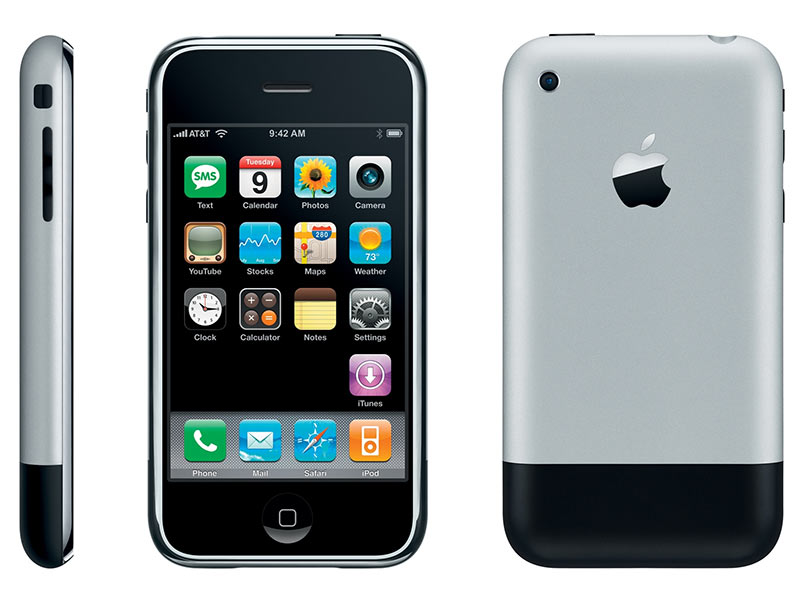
\includegraphics[width=0.5\textwidth]{../assets/img/Originele-iPhone.jpg}
            \caption*{Tout commence en juin 2007 avec l'iPhone.}
            \label{Fig:Originele-iPhone}
        \end{center}
    \end{figure}
\end{frame}

\subsection{Shopping time !}
\begin{frame}[fragile,t]{\secname : \subsecname}
    \begin{figure}
        \begin{center}
            
\includegraphics[width=0.8\textwidth]{../assets/img/android_and_apple.jpg}
            \caption*{L'App Store a ouvert en juillet 2008 et l'Android Market en octobre de la même année.}
            \label{Fig:android_and_apple}
        \end{center}
    \end{figure}
\end{frame}

\subsection{La situation}
\begin{frame}[fragile,t]{\secname : \subsecname}
    \begin{itemize}
        \item Développer pour les 2 plateformes;
        \item Si vous avez les moyens de développer une application, vous êtes l'enfant cool du quartier;
        \item Risques et des coûts élevés;
        \item Les coûts explosent car il faut maintenir plusieurs bases de code.
        \item Deux grandes tendances :
              \begin{itemize}
                  \item Natif;
                  \item Sites Web responsives.
              \end{itemize}
    \end{itemize}
\end{frame}

\subsection{L'essor des solutions web}
\begin{frame}[fragile,t]{\secname : \subsecname}
    \begin{itemize}
        \item Moins cher;
        \item Technologies plus matures;
        \item Merci HTML5 et aux WebViews;
        \item Par exemples : \href{https://cordova.apache.org}{Cordova}.
        \item Ces applications avaient souvent du mal à reproduire l'aspect et la convivialité des applications natives.
    \end{itemize}
\end{frame}

\subsection{Des solutions hybrides}
\begin{frame}[fragile,t]{\secname : \subsecname}
    \begin{itemize}
        \item En 2015 Facebook dévoile React Native;
        \item Une solution hybride
              \begin{itemize}
                  \item Même logique métier que celle du web ( JavaScript).
                  \item Utiliser un WebView, mais un système de rendu natif.
              \end{itemize}
        \item Le succès est énorme;
        \item Mais des améliorations sont possibles (voir nécessaire).
    \end{itemize}
\end{frame}


\section{Flutter}
\subsection{Flutter, c'est quoi ?}
\begin{frame}[fragile,t]{\secname : \subsecname}
    \begin{itemize}
        \item A software development toolkit, de Google;
        \item Permet de construire des applications multiplateformes;
        \item Des paquets, plug-ins et beaucoup de widgets;
        \item Flutter n'est pas un langage;
        \item Flutter utilise \href{https://dart.dev}{Dart} comme langage de programmation.
    \end{itemize}
\end{frame}

\subsection{Quelques forces}
\begin{frame}[fragile,t]{\secname : \subsecname}
    \begin{itemize}
        \item Flutter permet de compiler pour le Web,Android et IOS;
        \item Flutter est open source;
        \item Flutter utilise un langage récent \href{https://dart.dev}{Dart};
        \item Flutter permet le rechargement à chaud (\href{https://flutter.dev/docs/development/tools/hot-reload}{hot reload});
        \item Flutter \href{https://flutter.dev/docs/development/ui/widgets/material}{supporte nativement} le \href{https://material.io/design/guidelines-overview}{Material Design} de Google;
        \item Flutter permet de programmer des animations et transitions personnelles ou déjà existantes;
        \item Flutter permet le databinding;
        \item Les concepts de flutter sont proches de \href{https://developer.apple.com/xcode/swiftui/}{SwiftUI} et \href{https://developer.android.com/jetpack/compose}{Jetpack Compose}.
        \item Flutter permet de faire des applications accessibles;
    \end{itemize}
\end{frame}

\subsection{Quelques faiblesses}
\begin{frame}[fragile,t]{\secname : \subsecname}
    \begin{itemize}
        \item Ce n'est pas du développement natif;
        \item N'est pas adapté pour des jeux et/ou applications audios;
        \item N'est pas adapté pour des besoins très spécifiques de l'environnement Apple;
        \item Ne supporte pas watchOS, tvOS etc.
        \item C'est un pari sur l'avenir, la technologie est très récente.
    \end{itemize}
\end{frame}

\subsection{Quelques Exemples}
\begin{frame}[fragile,t]{\secname : \subsecname}
    \begin{figure}[H]
        \begin{center}
            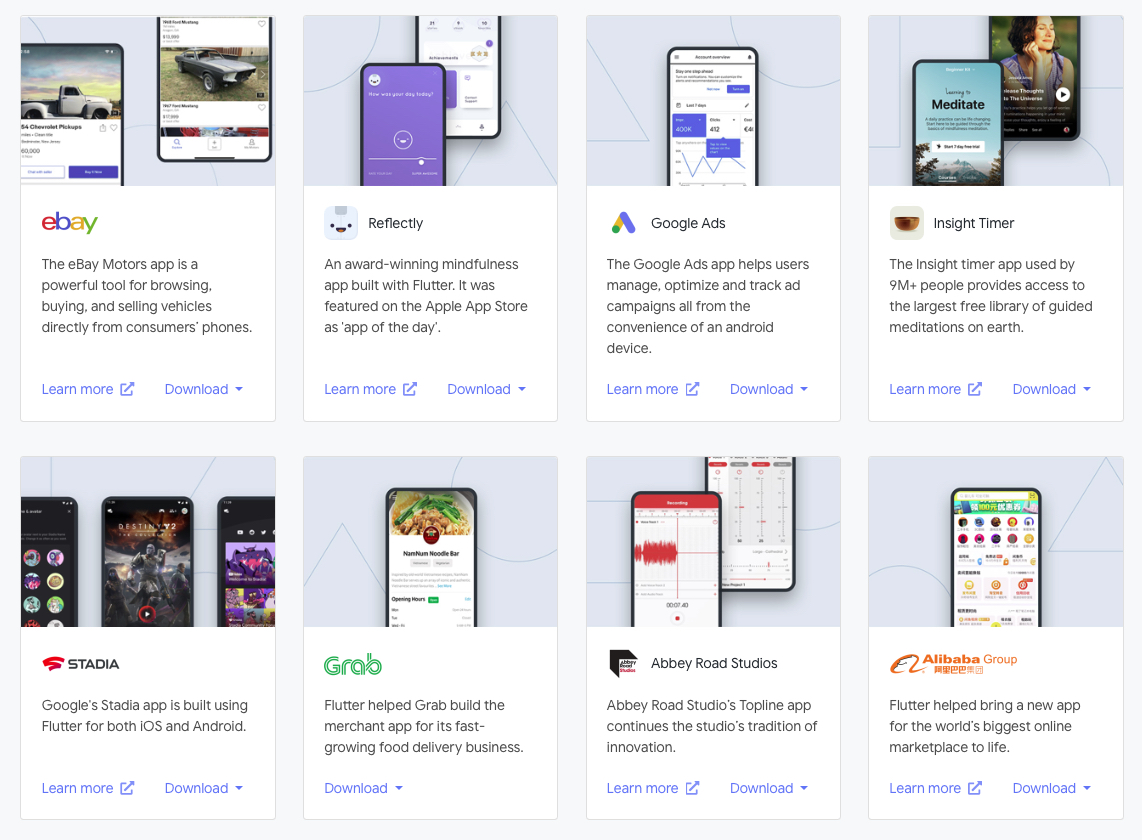
\includegraphics[width=0.7\textwidth]{../assets/img/exemples.jpg}
            \caption*{Quelques exemples parmi d'autres : \href{https://flutter.dev/showcase}{Apps take flight with Flutter}}
            \label{Fig:exemples}
        \end{center}
    \end{figure}
\end{frame}

\begin{frame}[fragile,t]{\secname : \subsecname}
    \begin{figure}[H]
        \begin{center}
            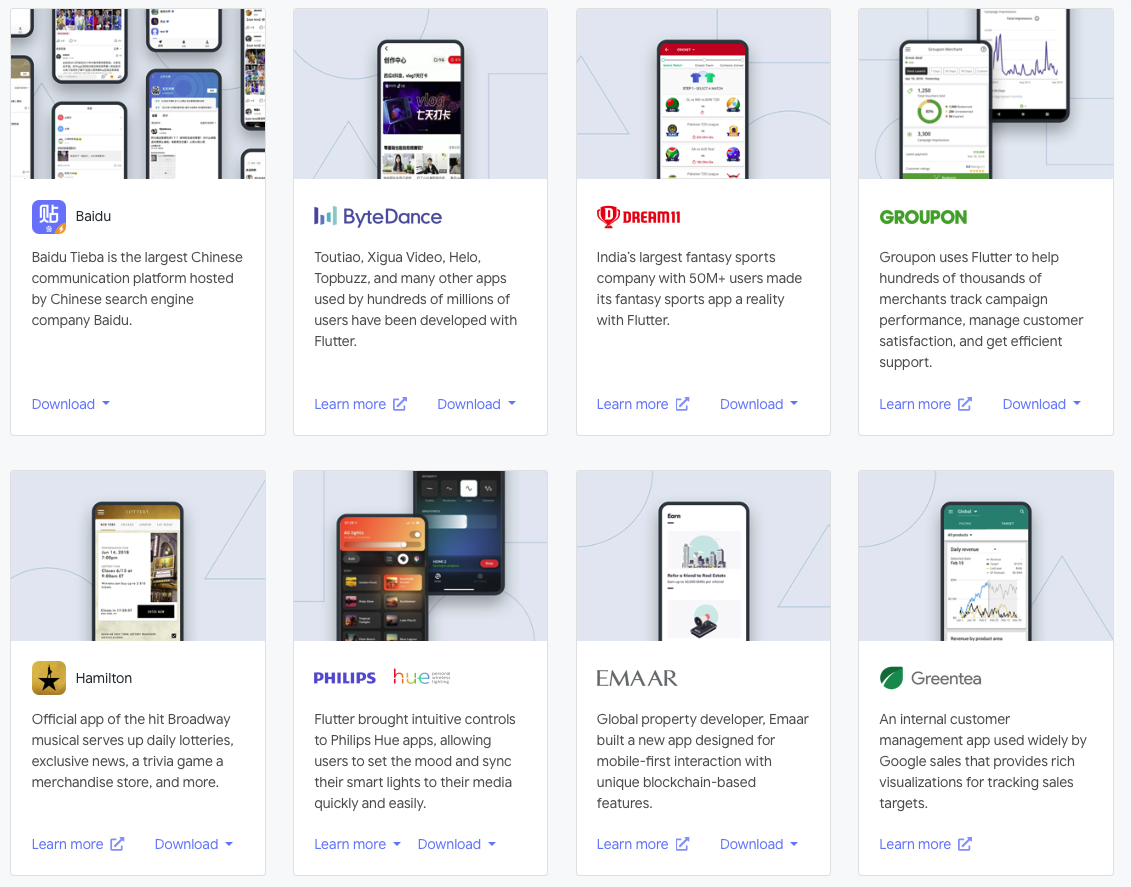
\includegraphics[width=0.7\textwidth]{../assets/img/exemples2.jpg}
            \caption*{Quelques exemples parmi d'autres : \href{https://flutter.dev/showcase}{Apps take flight with Flutter}}
            \label{Fig:exemples2}
        \end{center}
    \end{figure}
\end{frame}

\section{Architecture}

\subsection{Flutter}
\begin{frame}[fragile,t]{\secname : \subsecname}
    \begin{figure}[H]
        \begin{center}
            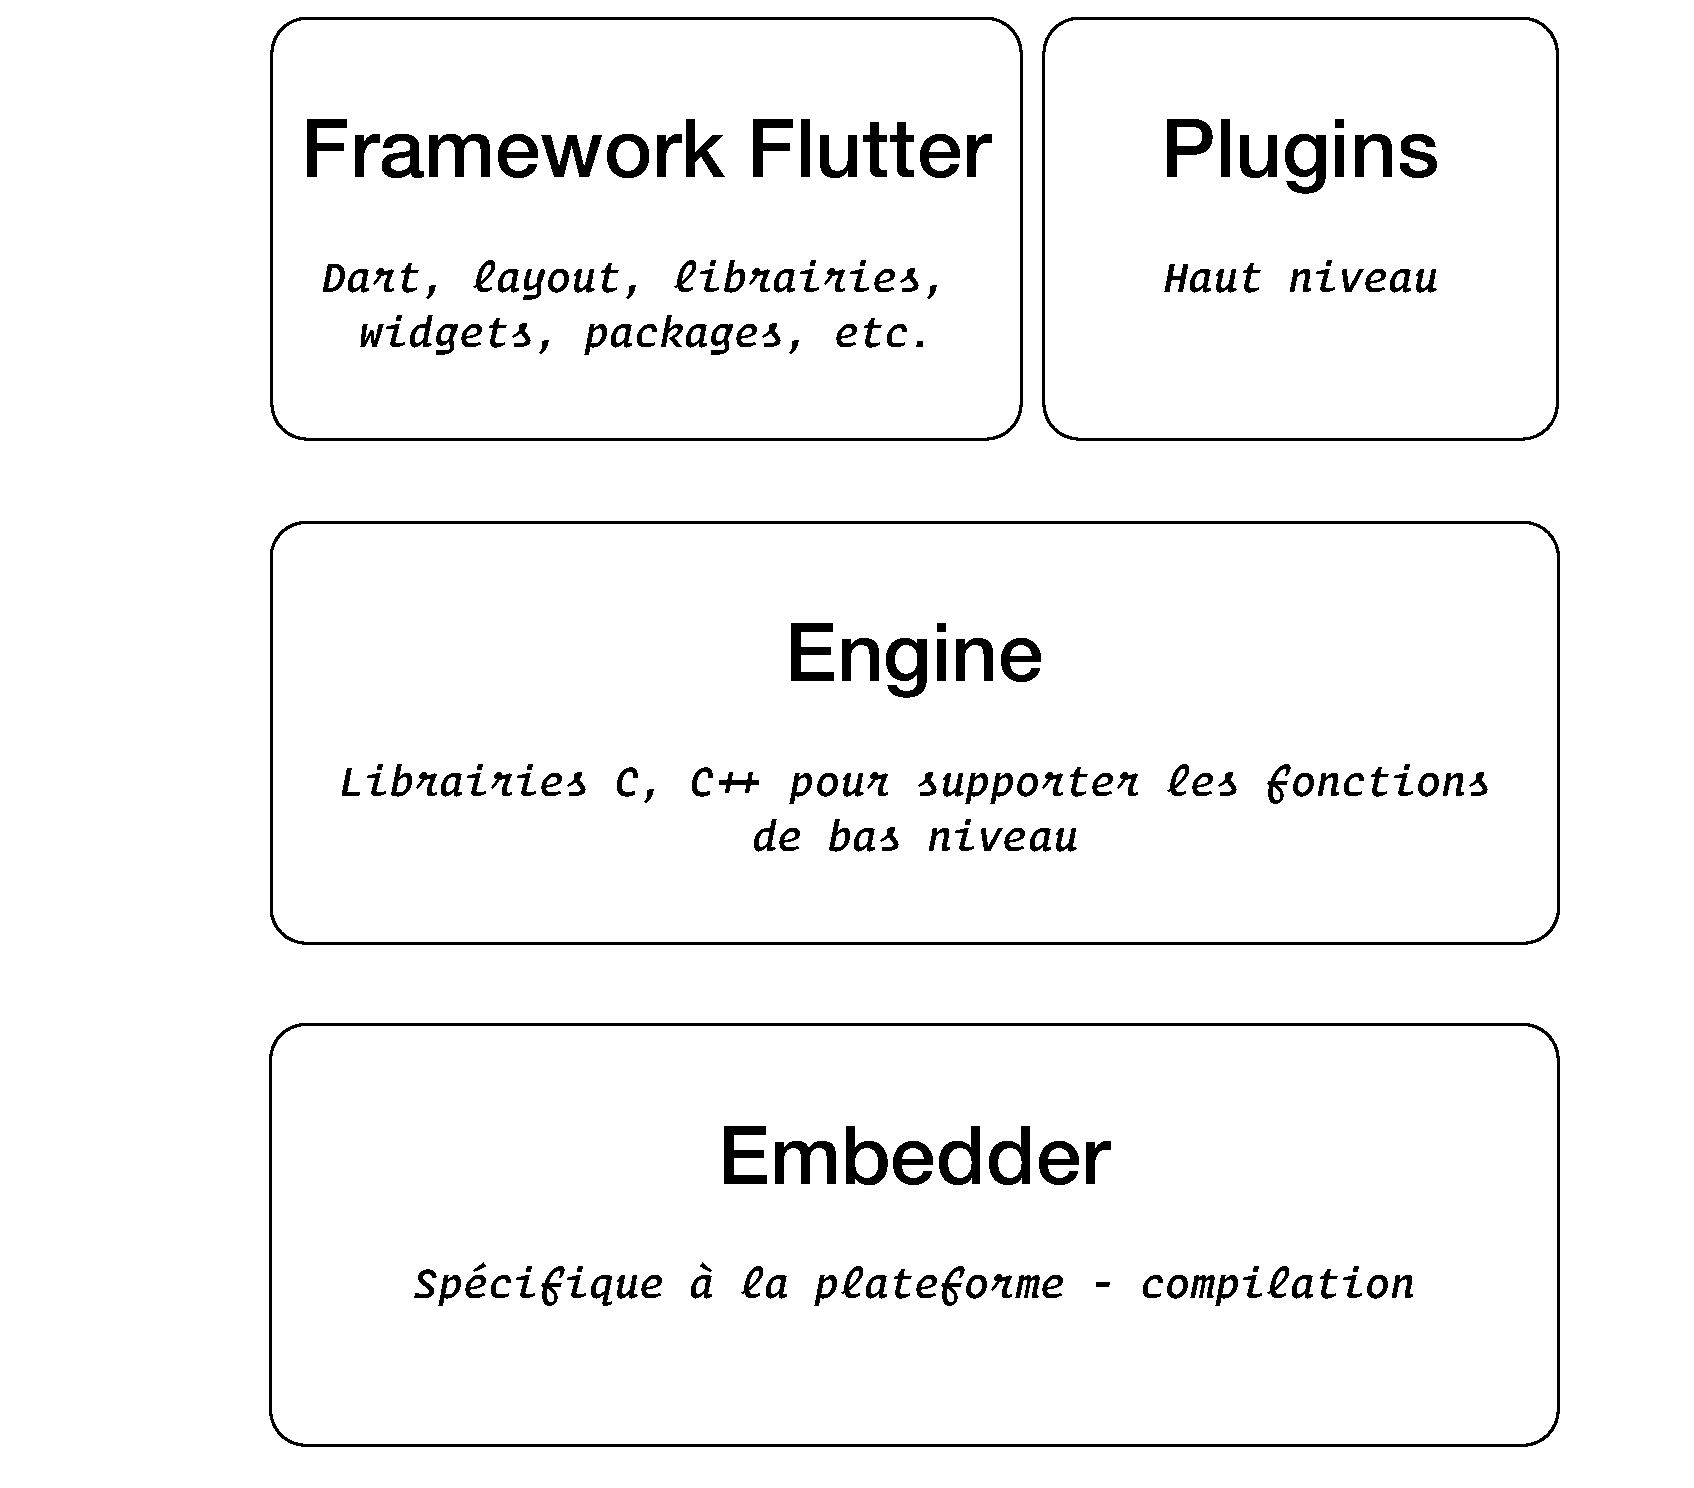
\includegraphics[width=0.5\textwidth]{../assets/img/architecture-flutter.eps}
            \caption*{Architecture Flutter \cite{raywenderlich2020flutter}}
            \label{Fig:architecture-flutter}
        \end{center}
    \end{figure}
\end{frame}

\subsubsection{Framework Flutter}
\begin{frame}[fragile,t]{\secname : \subsecname}
    \begin{itemize}
        \item Le \textbf{Framework Flutter} est écrit en Dart;
        \item Il contient des bibliothèques de haut niveau avec notamment :
              \begin{itemize}
                  \item Les thèmes;
                  \item Les widgets;
                  \item La mise en page;
                  \item Les animations.
              \end{itemize}
    \end{itemize}
\end{frame}
\subsubsection{Plug-ins}
\begin{frame}[fragile,t]{\secname : \subsecname}
    \begin{itemize}
        \item Les \textbf{Plugins} isolent des fonctionnalités de haut niveau :
              \begin{itemize}
                  \item La sérialisation JSON;
                  \item La géolocalisation;
                  \item L'accès aux caméras;
                  \item Les paiements in-app, etc.
              \end{itemize}
    \end{itemize}
\end{frame}

\subsubsection{Engine}
\begin{frame}[fragile,t]{\secname : \subsecname}
    \begin{itemize}
        \item La couche \textbf{Engine} contient les bibliothèques C++. Elle gère :
              \begin{itemize}
                  \item Les graphiques;
                  \item La mise en page du texte;
                  \item L'accessibilité;
                  \item L'architecture des plugins et le moteur d'exécution Dart.
              \end{itemize}
    \end{itemize}
\end{frame}

\subsubsection{Engine}
\begin{frame}[fragile,t]{\secname : \subsecname}
    \begin{itemize}
        \item L'\textbf{Embedder} est différent pour chaque plateforme cible. Il gère :
              \begin{itemize}
                  \item L'\textit{empaquetage} du code comme une application autonome.
              \end{itemize}
    \end{itemize}
\end{frame}

\begin{frame}[fragile,t]{\secname : \subsecname}
    \metroset{block=fill}
    \begin{block}{Remarque}
        Chacune des couches est encore une fois décomposée en plusieurs sous-couches.
    \end{block}
\end{frame}

\subsection{Découpe de la couche Framework}
\begin{frame}[fragile,t]{\secname : \subsecname}
    \begin{figure}[H]
        \begin{center}
            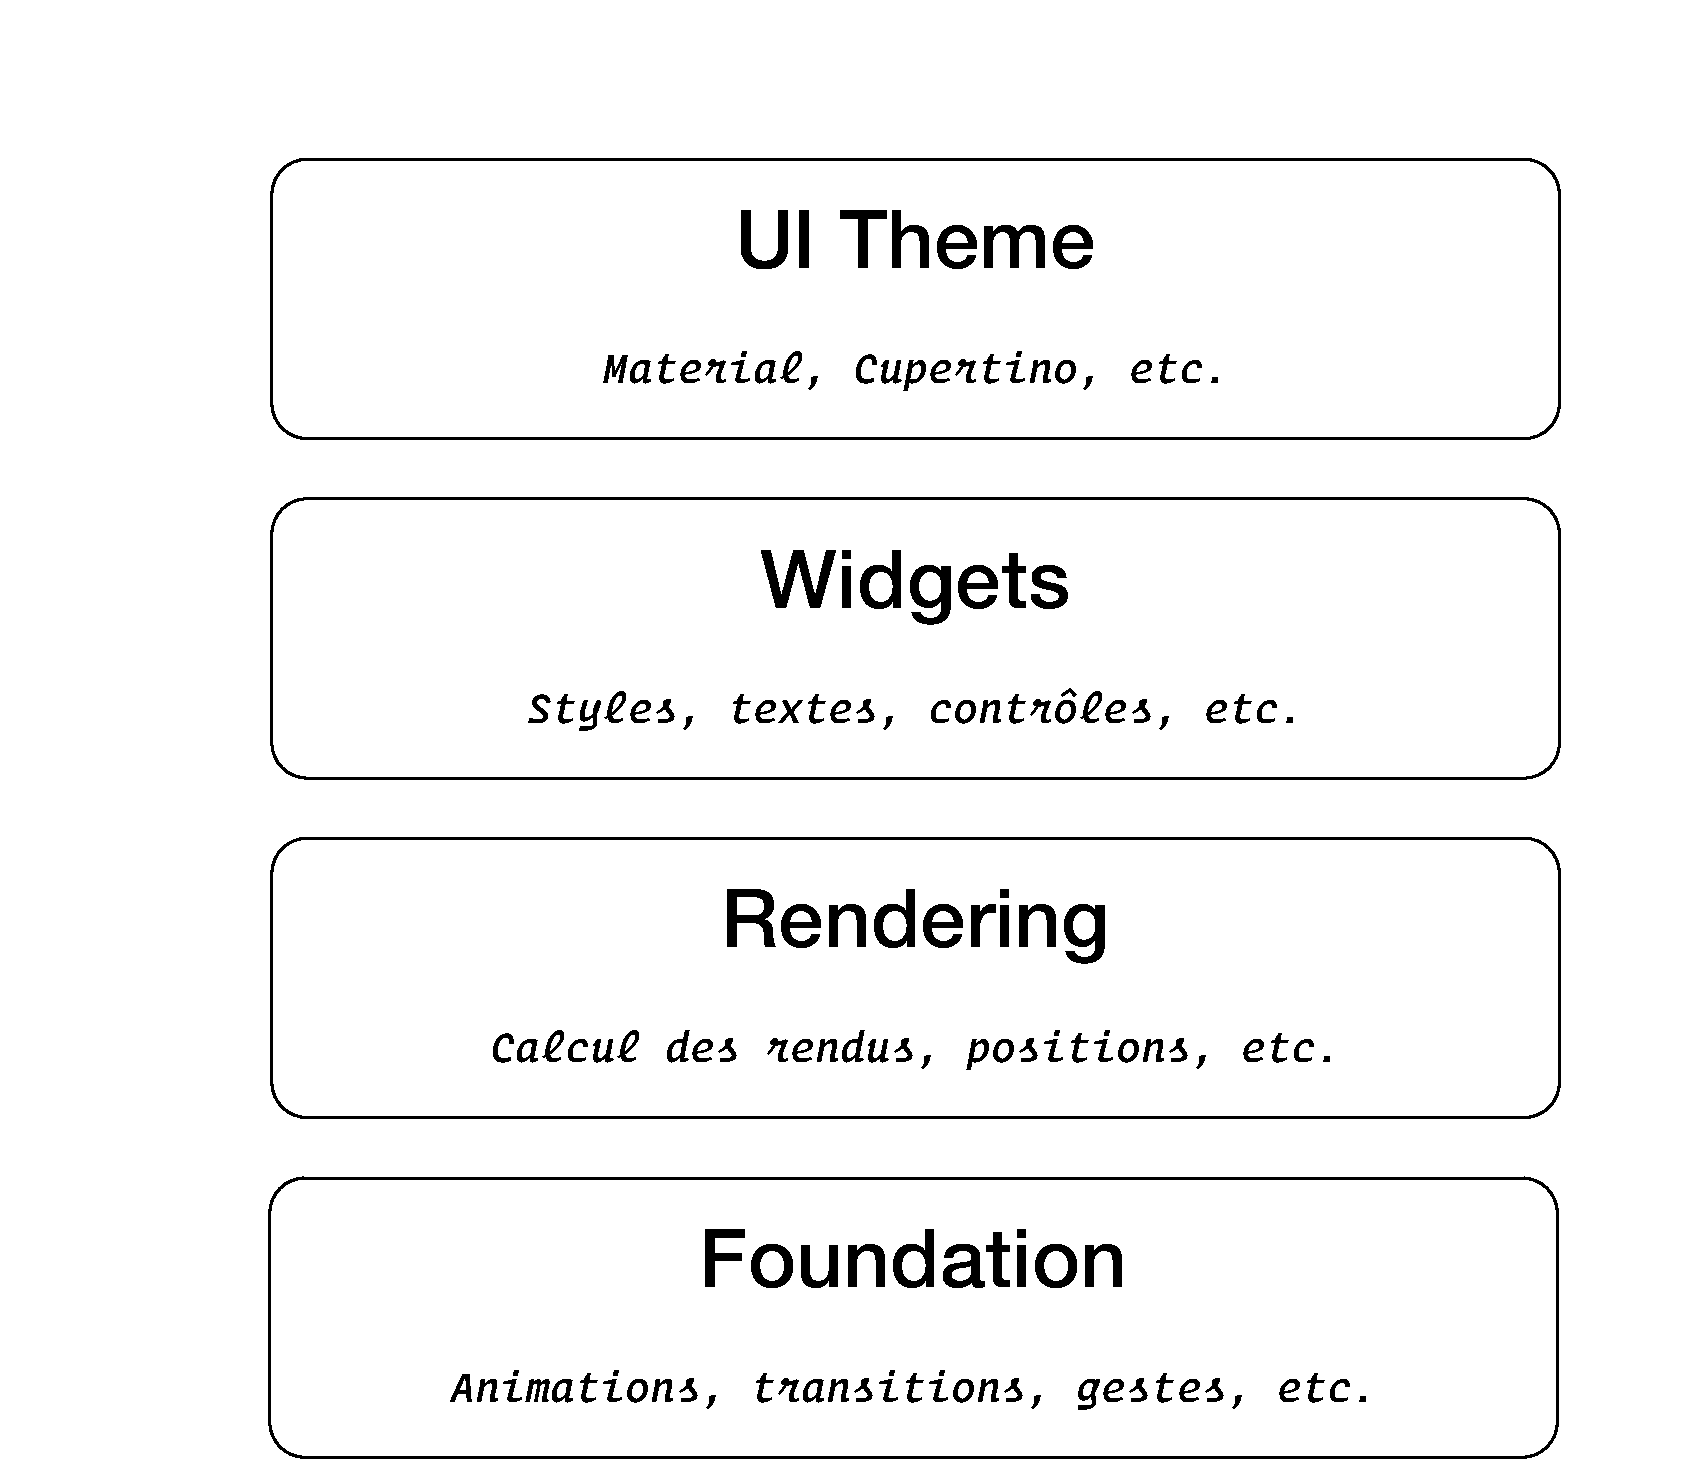
\includegraphics[width=0.5\textwidth]{../assets/img/architecture-framework.eps}
            \caption*{Architecture du framework Flutter \cite{raywenderlich2020flutter}}
            \label{Fig:architecture-framework}
        \end{center}
    \end{figure}
\end{frame}

\section{Installation}

\subsection{Liste des logiciels à installer}
\begin{frame}[fragile,t]{\secname : \subsecname}
    \begin{itemize}
        \item \href{https://flutter.dev/docs/get-started/install}{Flutter} SDK 2.2.0;
        \item \href{https://git-scm.com/downloads}{git} (si ce n'est déjà fait);
        \item \href{https://itunes.apple.com/us/app/xcode/id497799835}{Xcode} (si vous êtes sous macOS);
        \item \href{https://guides.cocoapods.org/using/getting-started.html#installation}{Cocoapods} (gestionnaire de dépendances que Flutter utilise);
        \item \href{https://developer.android.com/studio/install}{Android Studio};
        \item \href{https://www.jetbrains.com/fr-fr/idea/download/#section=mac}{IntelliJ IDEA} + Flutter Plugin;
        \item \href{https://code.visualstudio.com/download}{Visual Studio Code} (alternative à IntelliJ IDEA);
        \item \href{https://plugins.jetbrains.com/plugin/16602-embedded-dartpad}{Dartpad} (Tester des exemples Dart);
    \end{itemize}
\end{frame}

\subsection{Guide d'installation}
\begin{frame}[fragile,t]{\secname : \subsecname}
    \begin{center}
        \href{https://flutter.dev/docs/get-started/install}{GET STARTED !}
    \end{center}
    À l'issue du processus d'installation, vous devez depuis votre terminal être capable d’exécuter cette commande :
    \begin{lstlisting}[caption={Connaître la version de flutter},language=C, label=getversion]
    flutter --version
    \end{lstlisting}


\end{frame}

\subsection{Flutter Doctor}
\begin{frame}[fragile,t]{\secname : \subsecname}
    L’analyse de la commande \textit{flutter doctor} révèle plusieurs choses :
    \begin{itemize}
        \item Elle vérifie la version de Flutter actuellement installée.
        \item Elle vérifie que la licence Android permettant de développer sur des produits liés à cet OS est bien acceptée.
        \item Elle détecte la présence d’Android Studio et a vérifié que les plug-ins de Flutter (Flutter et Dart) sont bien installés.
        \item Elle détecte la présence d'un périphérique ou simulateur
    \end{itemize}
    \begin{lstlisting}[caption={Vérifier l'installation},language=bash, label=getversion]
        flutter doctor
        \end{lstlisting}
\end{frame}

\section{Première application}
\subsection{Création d'un nouveau projet}
\begin{frame}[fragile,t]{\secname : \subsecname}
    \begin{figure}[H]
        \begin{center}
            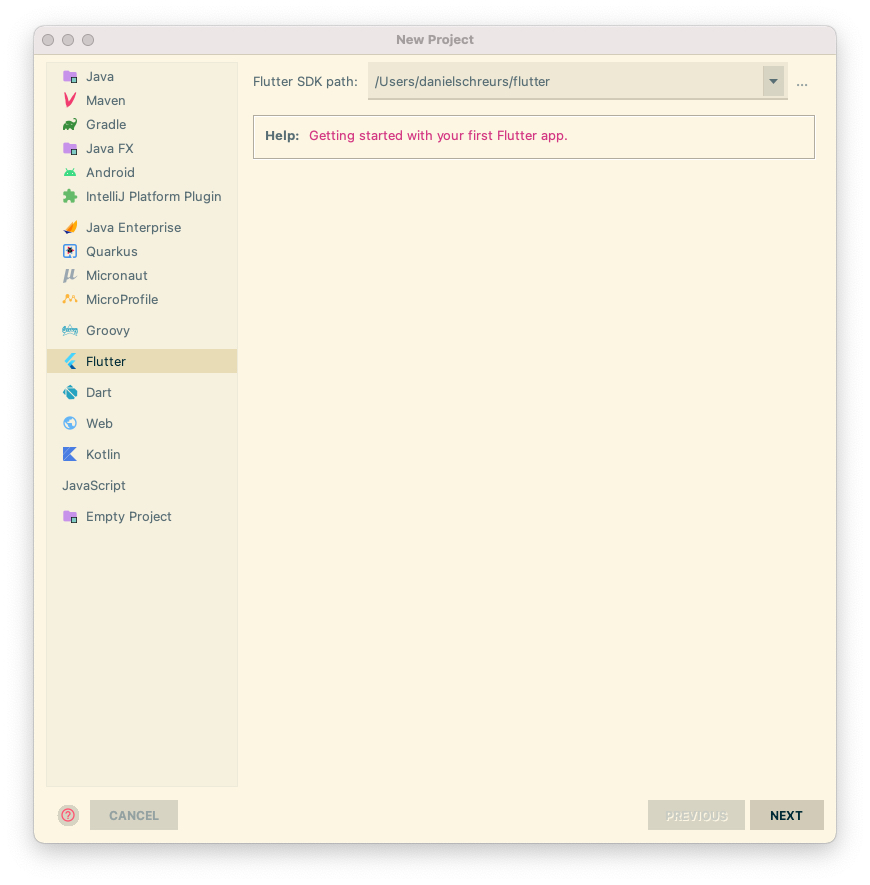
\includegraphics[width=0.4\textwidth]{../assets/img/new-project-1.jpg}
            \caption*{Création d'un nouveau projet Flutter depuis IntelliJ IDEA}
            \label{Fig:new-project-1}
        \end{center}
    \end{figure}
\end{frame}

\subsection{Configurer un nouveau projet}
\begin{frame}[fragile,t]{\secname : \subsecname}
    \begin{columns}
        \column{0.7\textwidth}
        \begin{figure}[H]
            \begin{center}
                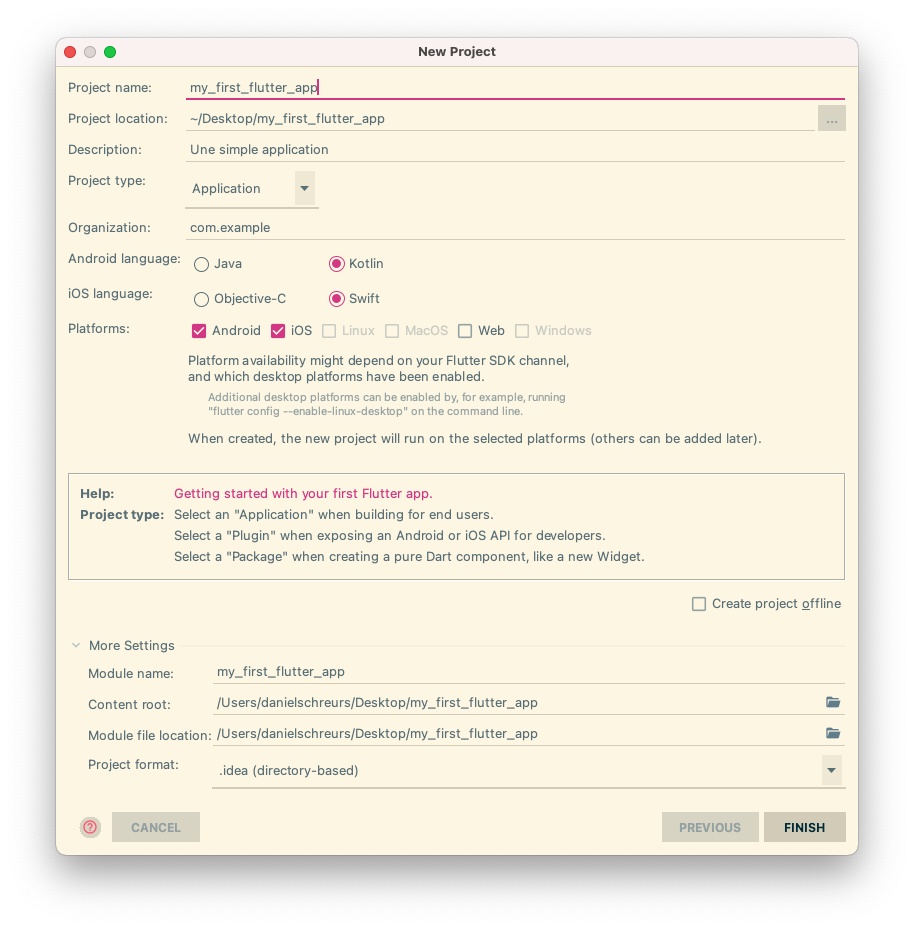
\includegraphics[width=0.6\textwidth]{../assets/img/new-project-2.jpg}
                \caption*{Configuration du nouveau projet Flutter depuis IntelliJ IDEA}
                \label{Fig:new-project-2}
            \end{center}
        \end{figure}
        \column{0.3\textwidth}
        \metroset{block=fill}
        \begin{block}{Remarque}
            Attention au $nom\_du\_projet$. Il faut suivre la convention $[a-z0-9\_]$ (\href{https://dart.dev/tools/pub/pubspec#name}{Documentation})
        \end{block}
    \end{columns}
\end{frame}

\subsection{Choisir un périphérique}
\begin{frame}[fragile,t]{\secname : \subsecname}
    \begin{figure}[H]
        \begin{center}
            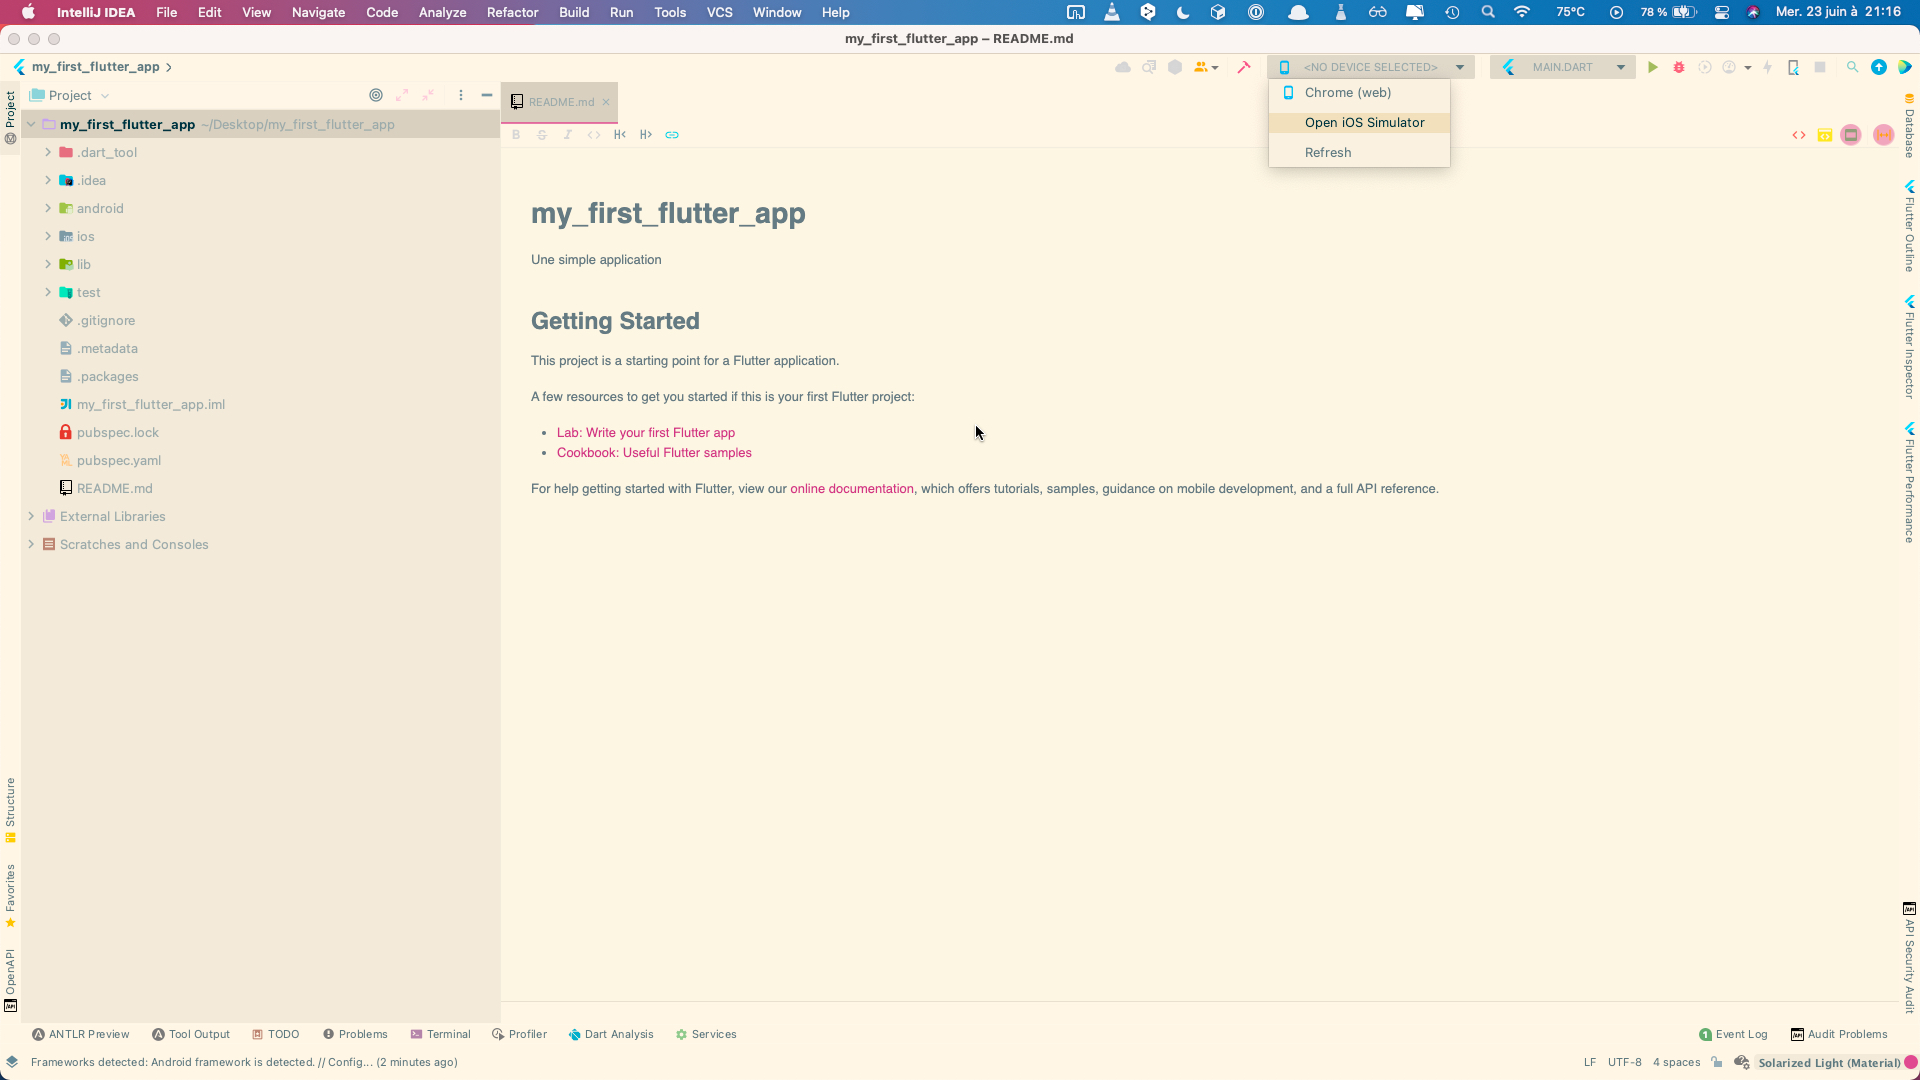
\includegraphics[width=0.85\textwidth]{../assets/img/new-project-3.jpg}
            \caption*{Demander à ouvrir un simulateur}
            \label{Fig:new-project-3}
        \end{center}
    \end{figure}
\end{frame}

\subsection{Lancer l'application}
\begin{frame}[fragile,t]{\secname : \subsecname}
    \begin{figure}[H]
        \begin{center}
            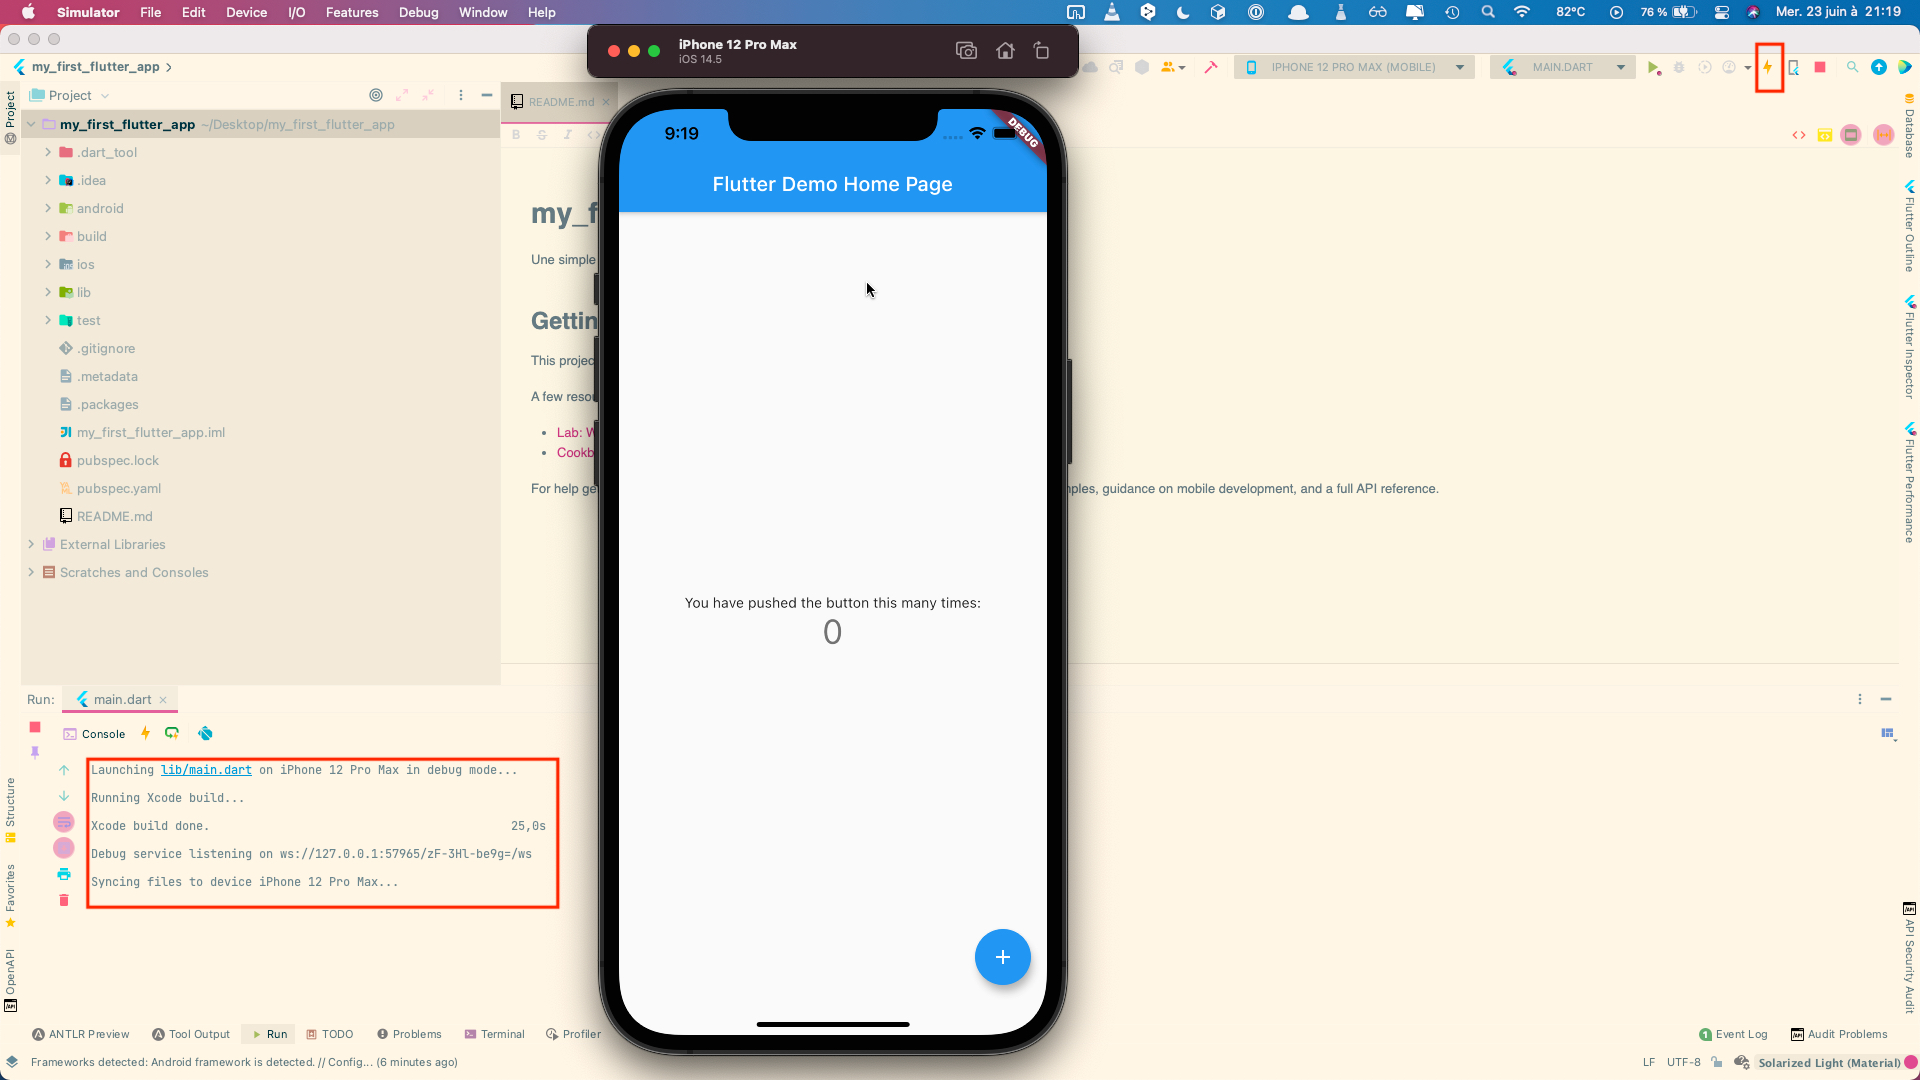
\includegraphics[width=0.85\textwidth]{../assets/img/new-project-5.jpg}
            \caption*{Démarrer l'application dans le simulateur}
            \label{Fig:new-project-5}
        \end{center}
    \end{figure}
\end{frame}

\subsection{En cas de problème}
\begin{frame}[fragile,t]{\secname : \subsecname}
    \begin{itemize}
        \item La documentation de Flutter : \href{flutter.dev}{flutter.dev}
        \item La documentation de Dart : \href{dart.dev}{dart.dev}
        \item Les autres : \href{https://flutter.dev/community}{flutter.dev/community}
        \item La chaine officielle sur YouTube : \href{https://www.youtube.com/c/flutterdev/}{youtube.com/c/flutterdev}
    \end{itemize}
\end{frame}


\begin{frame}[allowframebreaks]{References}
    \bibliography{ref}
    \bibliographystyle{abbrv}
\end{frame}

\end{document}